\chapter{Bayesian periodization of postembryonic CMZ activity}
\label{chap:CMZ}

\section{Preliminaries: Calculation of Bayesian evidence militates for independent log-Normal modelling of CMZ parameters}
To take up the question of how CMZ RPC activity evolves over time, we have collected observations of a variety of CMZ and retinal parameters derived from histological studies of cryosections of zebrafish eyes harvested over the first year of the animal's life. We wish to extract as much information as possible about the structure and time-evolution of the CMZ population as a whole, in order to know how to best model its constituent RPCs. The initial approach here will be to estimate parameters of the whole-eye CMZ from sample cryosections, and to use these estimates as the dataset which will inform our selection of appropriate models.

While it remains common to assume that population data are normally distributed, and so simply to calculate means and standard deviations as the statistical representation of the underlying population, it has been known for decades \cite{Heath1967} that log-normal distributions are usually better models of the outcomes produced by additive processes with small, variable steps (like population sizes or income distributions). We therefore start with the selection of appropriate models for the CMZ- and retina-level population measurements critical to the inferences that follow.

As a first pass at this question, we calculate the likelihood ratio for the hypothesis that the parameter measurements, and the calculated quantities derived from them, are log-normally distributed against the the one that they are simply normally distributed. These results are displayed in Table \ref{PLHRtable}

\begin{table}[!ht]
    \centering
    \caption{
    {\bf Likelihood ratio comparison between normal and log-normal models of retinal population parameters}}
    \begin{tabular}{|l|l|l|l|}
    \hline
    {\bf Parameter} & {\bf $\mathcal{N}$ logLH} & {\bf Log-$\mathcal{N}$ logLH} & {\bf logLR} \\ \hline
    Sectional PCNA+ve & -285.611 & {\bf -283.214} & 2.397\\ \hline
    Lens diameter & {\bf -203.102} & -203.854 & -0.752\\ \hline
    CMZ annular pop.($\dagger$)  & -484.768 & {\bf -482.733} & 2.035\\ \hline
    RPE length & {\bf -368.232} & -368.609 & -0.377\\ \hline
    CR thickness ($\dagger$) & {\bf -240.858} & -241.032 & -0.174\\ \hline
    CR volume ($\dagger$) & -1091.615 & {\bf -1091.146} & 0.469\\ \hline
    \end{tabular}
    \begin{flushleft} $\mathcal{N}$: Normal distribution. logLH: logarithm of p(D|M), the likelihood of the data given the model. logLR: logarithm of the likelihood ratio; positive ratios in favour of the log-$\mathcal{N}$ model. Superior likelihoods are bolded. $\dagger$: Calculated quantities. Sectional PCNA+ve: population of PCNA-positive CMZ RPCs per 14$\mu$m cryosection. CMZ annular pop: population of annular CMZ. RPE: retinal pigmented epithelium. CR: cellular retina.
    \end{flushleft}
    \label{PLHRtable}
\end{table}

These results suggest that the organism-level population distribution of eye-level CMZ population counts, as assayed by PCNA immunostaining, is better modelled log-normally than normally. This is true whether we test the primary per-section count meaurements, or the estimated whole-annulus population, calculated as described in \autoref{sec:lenspopest}, even though this quantity is calculated using the normally-distributed lens diameter\footnote{The apparent superiority of the normal model for lens diameter may be due to the paucity of data at later time points; as described in INSERT METHODS AUTOREF, lenses are difficult to retain in this histological context.}. The most likely log-Normal representations of the CMZ populations are about two orders of magnitude more likely than the Normal alternative. Additionally, although normal models are slightly favoured for describing the population-level distributions of RPE length and cellular retina thickness, the derived cellular retina volume quantity is better modeled by a log-Normal distribution. As the two calculated quantities will be the primary ones used in our inferences about population-level CMZ dynamics, we are most concerned with these measures; at this point, the log-Normal distribution looks to be more informative for both.

We have emphasized the danger of relying overmuch on the parameterisation of single most-likely model fits in \autoref{chap:SMMEoutro}, which is what the simple likelihood ratios above represent: the joint likelihood of the maximum a posteriori distribution fitted to the measurements taken from each age cohort. Since the choice of model describing the estimated annular population and retinal volume is critical to the success of later inferences, we used Galilean Monte Carlo-Nested Sampling (GMC-NS) to estimate the Bayesian evidence (the marginal probability of the data over all model parameterisations) for these hypotheses. Although it is very unlikely that GMC-NS will result in conclusions from the likelihood ratio, this simple test serves to prove the function of the \path{GMC_NS.jl} package, and demonstrate the inferential logic. Evidence estimates and ratios are presented in Table \ref{PZRtable}.

\begin{table}[!ht]
    \centering
    \caption{
    {\bf Evidence favours log-normal models of retinal population parameters}}
    \begin{tabular}{|l|l|l|l|l|}
    \hline
    {\bf Parameter} & {\bf $\mathcal{N}$ logZ} & {\bf Log-$\mathcal{N}$ logZ} & {\bf logZR} & {\bf $\sigma$ significance}\\ \hline
    CMZ Population & -43982.0 $\pm$ 31.0 & -5527.2 $\pm$ 9.9 & 38454.0 $\pm$ 33.0 & 1180.2\\ \hline
    Estimated Retinal Volume & -16651.0 $\pm$ 18.0 & -15226.0 $\pm$ 16.0 & 1424.0 $\pm$ 24.0 & 59.0\\ \hline
    \end{tabular}
    \begin{flushleft} $\mathcal{N}$: Normal distribution. logZ: logarithm of p(D), the marginal likelihood of the data, or model evidence. logZR: evidence ratio; positive ratios in favour of the log-$\mathcal{N}$ model. Largest evidence values bolded. CR: cellular retina.
    \end{flushleft}
    \label{PZRtable}
\end{table}

Unsurprisingly, full estimation of the Bayesian evidence for the Normal vs. log-Normal hypotheses for our calculated parameters produces the same basic story as the rough calculation of likelihood ratio from the single-fit MAP models. There are approximately 38000 orders of magnitude more evidence for the log-Normal model of interindividual variation in estimated CMZ annulus RPC population over time. This result has greater than 1180 standard deviations of significance\footnote{The typical standard for a "discovery" in particle physics is >5$\sigma$ \cite{Lyons2013}. Assuming Normally distributed error, the probability that the models were, in fact, equally good at 3 standard deviations of significance would be about a tenth of a percent (i.e. .001). At 10 standard deviations the figure is \num{7.62e-24}. Assuming the sample is representative, we have nigh certainty about these results and no reason to pursue the matter further.}. There are approximately 1400 orders of magnitude more evidence for the log-Normal model for the variability in the cellular retinal volume estimate, with 59 standard deviations of significance. Based on these results, we need not have any compunction about modelling population outcomes for these parameters with log-Normal distributions, as the evidence supplied by our observations plainly supports it.

If between-individual variation in retinal CMZ population and retinal volume are both well-modelled log-normally, the question of their independence immediately arises. It seems plausible that the size of the CMZ population would be roughly proportional to the overall volume of the retina, upon central specification, and establishment of the peripheral CMZ remnant. Moreover, since the growth of retinal volume over the life of the organism is driven primarily by the CMZ\footnote{One observes occasional proliferative clusters in the central retina throughout the life of the fish; these are typically ascribed to M\"{u}ller glial repair processes. I am unaware of any estimate as to the relative contribution of these clusters vs. the CMZ. As we shall see, there is probably more turnover in the specified retina than previously believed. As a result, the relative contribution of these central clusters should probably be subject to statistical estimation; they may be more significant than mere lesion-repair sites.}, it seems likely that either the retinal growth rate is well correlated with the size of the CMZ. Since both of these questions bear upon the manner in which we model the CMZ, we performed Bayesian model selection by the so-called Empirical Bayes method for linear regression, which provides for direct estimation of the evidence for models consisting of linear equations of variables \cite{Bishop2006}.

We find that individual CMZ population and retinal volume estimates are better described by uncorrelated models at in all ages, with the exception of 23.0 dpf. It is interesting to note that the evidence in favour of non-correlation is weakest between 17 and 30 dpf. These data are displayed in \autoref{corrtable}. Of particular importance are the data for 3dpf embryos, as we intend to seed model retinae with CMZ populations and volumes drawn from these distributions. The data for these animals are plotted in \autoref{gausscorrelation}. The general lack of correlation between CMZ population and retinal volume estimates may be due to the loss of information involved in the estimation calculations; on the other hand, it is more plausible that CMZ population should be associated with the rate of retinal volume growth rather than the volume of the retina itself, which suggests that the rate of retinal contribution from the CMZ is probably highest between 17 and 23 days. Because growth rate data are unavailable for single individuals, we cannot make this inference directly.

\begin{table}[!ht]
    \centering
    \caption{{\bf Evidence favours uncorrelated linear models of CMZ-population and retinal volume over time}}
    \begin{tabular}{|l|l|l|l|}
        \hline
        {\bf Age (dpf)} & {\bf Uncorrelated logZ} & {\bf Correlated logZ} & {\bf logZR}\\ \hline
        3.0 & {\bf -87.651} & -91.902 & 4.252\\ \hline
        5.0 & {\bf -90.0} & -92.362 & 2.362\\ \hline
        8.0 & {\bf -90.918} & -96.013 & 5.095\\ \hline
        12.0 & {\bf -91.183} & -99.049 & 7.866\\ \hline
        17.0 & {\bf -94.818} & -96.668 & 1.85\\ \hline
        23.0 & -103.386 & {\bf -103.219} & -0.167\\ \hline
        30.0 & {\bf -103.511} & -104.092 & 0.581\\ \hline
        60.0 & {\bf -115.025} & -118.169 & 3.144\\ \hline
        90.0 & {\bf -113.533} & -122.427 & 8.894\\ \hline
        180.0 & {\bf -116.778} & -124.547 & 7.769\\ \hline
        360.0 & {\bf -121.016} & -128.637 & 7.621\\ \hline
        \end{tabular}
    \begin{flushleft} logZ: logarithm of p(D), the marginal likelihood of the data, or model evidence. logZR: evidence ratio; positive ratios in favour of the uncorrelated model. Largest evidence values bolded.
    \end{flushleft}
    \label{corrtable}
\end{table}

\begin{figure}[!h]
    \makebox[\textwidth][c]{\includegraphics[width=.75\textwidth]{cmz/3dcorr.png}}    
    \caption{{\bf CMZ population and retinal volume estimates are uncorrelated at 3dpf}}
    Individual CMZ population estimate vs retinal volume estimate for 3dpf animals. Uncorrelated and correlated linear models of these variables are plotted as the mean$\pm$95\% CI of the predictive distribution of the fitted model.
    \label{gausscorrelation}
\end{figure}

From these analyses, we conclude that organismal variability in the CMZ population and retinal volume estimates are best described by independent log-Normal distributions. Because log-Normal distributions are simply transformed Normal Gaussian distributions, we may model our uncertainty about their parameters with Normal-Gamma distributions over the mean and variance of the underlying Normal distribution of the log-Normal population model ("the underlying"). That is, our prior and posterior belief about the relative likelihood of values of the mean of the underlying may be modelled with a Normal distribution, and our beliefs about its variance with a Gamma, such that our joint uncertainty is the product of the two distributions. This is explained in more detail in \autoref{sec:NormalGamma}. A useful analytic feature of the Normal-Gamma prior is that the marginal posterior distribution of the mean, assuming an uninformative (ignorance) prior, is a location-scaled T distribution; this is so because the weighted sum of an infinite series of Normal distributions (i.e. the likelihood-weighted sum of all the Normal distributions that could underly the log-Normal models), is a T distribution. T distributions are notably more resistent to outlier distortion than Normal distributions themselves are, and may be estimated with as few as two observations, making them highly flexible. Most of the descriptive statistics in the next section, therefore, calculate the credible interval for the posterior mean of the underlying by T distributions (with the correct change of variables by exponential transformation to produce the features of the correct log-Normal distribution). Unfortunately, differences of T distributions are not, themselves, necessarily T-distributed, so we have relied on Monte Carlo estimation of rates of change of the these posterior means over time. With our log-Normal models selected, and the descriptive tool of the posterior mean T distribution in hand, we turn now to a survey of the zebrafish CMZ in the first year of life.

\section{Survey of CMZ population and gross retinal contribution}

If it is true that the majority of zebrafish retinogenesis occurs postembryonically, and that models trained on embryonic data do not describe this period well, what characterises this CMZ-driven phase of retinogenesis? We begin by presenting our estimates of individual CMZ annulus population and retinal volume over the first year of life, in \autoref{CMZoverall}, panels A and C.

\begin{figure}[!h]
    \makebox[\textwidth][c]{\includegraphics[width=1.\textwidth]{cmz/CMZoverall.png}}    
    \caption{{\bf Population and activity of the CMZ over the first year of \textit{D.rerio} life}}
    Panel A: Marginal posterior mean CMZ annulus population. Panel B: Marginal posterior mean retinal volume estimate. Insets in Panels A \& B display data from 3-17 dpf. Panel C: Marginal posterior mean of the proliferative index of the CMZ annulus, assayed by specified retinal neurons with incorporated thymidine from an 8hr pulse at the indicated ages. Panel D: Mean daily rate of volumetric increase of the neural retina, calculated as the difference in volumes between two ages over the number of elapsed days. All means are displayed in a band representing the $\pm 95 \%$ credible interval for the marginal posterior distribution of the mean.
    \label{CMZoverall}
\end{figure}

An initial, relatively quiescent period in the population history of the CMZ can be inferred from the lack of growth observed in the first week of life, as well as the observations presented in \autoref{rysCycle}, which demonstrate that CMZ RPCs are proliferating too slowly to be labelled by a day's pulse of a thymidine analogue at 5dpf in the wild-type and heterozygote siblings of npat mutants. Interestingly, we have good confidence that retinal volume continues to grow over this time; 99.56\% of the marginal posterior mass of the mean 5dpf estimate is above the 3dpf mean, suggesting that this proliferative pause is too short to appear in the retinal volume data.

In any case, the first two to three weeks of life (magnified in lens insets in panels A and C) appear to mark a relatively slow build in both estimated CMZ annulus population and retinal volume compared to the explosion which follows immediately thereafter. While zebrafish are better staged by size than age \cite{Parichy2009}, the onset of this explosive growth seems to come somewhat earlier than the typical metamorphic transition from larval to juvenile stages at ~45dpf \cite{Singleman2014}. This raises the question of the manner in which the CMZ contributes to the retina during the critical period of exponential growth of the organism, between about 45 and 90dpf. It is plausible, for instance, that the growth of the CMZ population mainly reflects the increased output of stem cells, with RPCs specifying at some steady rate, or that the CMZ builds itself up for a wave of specification somewhat later, similarly to the sequence of events in the embryonic central retina.

In order to get a better sense of this timing, we simulated the mean daily rate of CMZ annulus population and retinal volume change, by performing Monte Carlo difference operations between samples from the marginal posterior means of subsequent timepoints. These simulated mean rates and their associated confidence intervals are plotted in \autoref{CMZoverall} panels B and D. These show the basic time-structure of the phenomenon; the large increase in simulated daily CMZ population growth rate occurs before the large increase in retinal volume, but the CMZ population estimate does not begin to drop off until 60dpf, by which time the majority of volumetric growth is complete. This seems to substantiate some combination of the scenarios outlined above: there is an early buildup of CMZ population around 18-30dpf, before CMZ RPCs begin to make their primary contribution to the retina between 30-60dpf, which is characterised by much slower population growth and more rapid volumetric growth, implying steady and elevated specification of RPCs. The greater uncertainty associated with our population estimates, relative to their magnitude, results in correspondingly less certainty about the size of the population growth rate spike. For instance, we calculate a >99\% probability that the mean retinal volumetric rate growth peak at 60 dpf is at least 6-fold greater than the mean at 30dpf. By contrast, only about 97\% of the posterior mean density of  the population growth rate at the 23d peak (230.2 $\frac{cells}{d}$) is greater than the mean at 3dpf, which is a small negative value (-5.5 $\frac{cells}{d}$). 

Subsequent to the bulk of the CMZ buildup and contribution to the retina, the population of the CMZ declines at about 39\% the rate of its peak ascent, with an estimated -90.1$\frac{cells}{d}$ by 90dpf. This process thins out the CMZ population to below its size immediately after embryogenesis, spread out over a much larger peripheral annulus, for a much less dense mature CMZ. Interestingly, the 95\% CI on the marginal posterior mean of estimated retinal volume at 180 dpf (\SI{1.10(4)E9}{\cubic\micro\metre}) completely encompasses the 95\% CI on volume at 90dpf (\SI{1.11(3)E9}{\cubic\micro\metre}), while we assess a 99.6\% probability of the 360dpf mean (\SI{1.73(10)E9}{\cubic\micro\metre}) being greater than 180dpf. This suggests a possible second period of quiescence from approximately 90-180dpf, followed by steady contribution to the retina without a buildup in the CMZ population subsequently.

Given this rough description, it seems obvious that the ontogeny of the CMZ as a stem cell niche is characterised by different phases of activity, with different rates of proliferation and specification. It is not immediately clear what sort of periodization is justified by the data. It seems plausible that as few as two phases could explain the data well enough: an initial phase of logarithmic growth, with short cell cycle time and lower exit rate of RPCs from the CMZ into the specified neural retina, followed by a second phase of decay with longer cycle time and higher exit rate. On the other hand, perhaps some of the data features noted above justify a more bespoke model that captures, for instance, the initial quiescent period, or the post-180dpf growth of the retina. Because this is straightforwardly a question of how much model structure is justified by our data, we may address it as a model selection problem, using the system of Bayesian inference provided by nested sampling, and it is to this we now turn.

\section{Periodization of postembryonic CMZ activity by Galilean Monte Carlo Nested Sampling}

To perform our model selection task, we wish to simulate the time-evolution of CMZ population and retinal volume. This requires us to supply initial values for the size of the simulated CMZ populations and the volumes of the simulated retinae they are associated with. Given the findings presented in \autoref{gausscorrelation}, we are justified in initializing CMZ population and retinal volume by independent samples from the log-Normal models of their interindividual variability at 3dpf, at the end of embryogenesis and the beginning of CMZ-driven retinal growth. In order to produce new, simulated values of CMZ population and retinal volume, we apply a system of difference equations as follows, where $pop_n$ is the population at $n$ dpf, $CT$ is the mean cell cycle time of the population in hours, and $\epsilon$ is the proportion of the population at time $n-1$ that exits cycle and contributes to the volume of the specified neural retina, and $\mu_{cv}$ is the mean volume per cell contributed to the retina in \si{\cubic\micro\metre}:

\begin{equation}
    p_n=p_{n-1} \cdot 2^{\frac{24}{CT}} - p_{n-1} \cdot \epsilon
    \label{popeq}
\end{equation}

\begin{equation}
    v_n=v_{n-1} + p_{n-1} \cdot \epsilon \cdot \mu_{cv}
    \label{voleq}
\end{equation}

A model "phase" can then be defined by the $CT$ and $exit$ parameters it applies to update the population and volume over its length. The full parameterisation of a model with $p$ phases is given by $p$ pairs of $CT$ and $exit$ values, $p-1$ phase transition times, and $\mu_{cv}$, which is taken to apply equally to all phases. Given an initial population and volume sampled from the log-Normal models of their interindividual distributions, \autoref{popeq} and \autoref{voleq} may be applied to these values difference equations can be applied to produce simulated sample values at the times actually observed. Many such samples obtained by Monte Carlo can be used to estimate log-Normal distributions for the model parameters, which can be used to score the model against observations. By defining prior distributions over the model parameters, we may sample from the prior to initialize a model ensemble. The ensemble can then be compressed by nested sampling, moving each model-particle over the parameter space by Galilean Monte Carlo, as described in \autoref{GMC}. Using the typical procedures applied in nested sampling \cite{Skilling2006}, we calculated the Bayesian evidence for each of 1, 2, and 3-phase models. These results are presented in, with output from maximum a posteriori parameterizations for each model plotted against observations in.

\begin{figure}[!h]
    \makebox[\textwidth][c]{\includegraphics[width=1.\textwidth]{cmz/a10pMAP.png}}    
    \caption{{\bf Population and activity of the CMZ over the first year of \textit{D.rerio} life}}
    Panel A: Marginal posterior mean CMZ annulus population. Panel B: Marginal posterior mean retinal volume estimate. Insets in Panels A \& B display data from 3-17 dpf. Panel C: Marginal posterior mean of the proliferative index of the CMZ annulus, assayed by specified retinal neurons with incorporated thymidine from an 8hr pulse at the indicated ages. Panel D: Mean daily rate of volumetric increase of the neural retina, calculated as the difference in volumes between two ages over the number of elapsed days. All means are displayed in a band representing the $\pm 95 \%$ credible interval for the marginal posterior distribution of the mean.
    \label{CMZoverall}
\end{figure}

\begin{figure}[!h]
    \makebox[\textwidth][c]{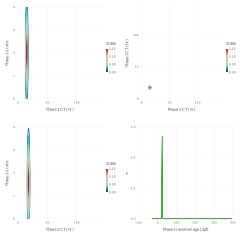
\includegraphics[width=1.\textwidth]{cmz/a10pmarginals.svg}}    
    \caption{{\bf Population and activity of the CMZ over the first year of \textit{D.rerio} life}}
    Panel A: Marginal posterior mean CMZ annulus population. Panel B: Marginal posterior mean retinal volume estimate. Insets in Panels A \& B display data from 3-17 dpf. Panel C: Marginal posterior mean of the proliferative index of the CMZ annulus, assayed by specified retinal neurons with incorporated thymidine from an 8hr pulse at the indicated ages. Panel D: Mean daily rate of volumetric increase of the neural retina, calculated as the difference in volumes between two ages over the number of elapsed days. All means are displayed in a band representing the $\pm 95 \%$ credible interval for the marginal posterior distribution of the mean.
    \label{CMZoverall}
\end{figure}


\section{Characterisation of asymmetrical CMZ population and retinal contribution dynamics}

In the course of the preceding investigations, it became apparent that the population asymmetry mentioned in \autoref{chap:SMMEoutro} was not a static phenomenon, with the dorsal lobe of the CMZ annulus being consistently more populous than the ventral lobe, as generally implied by the sources covered in \autoref{chap:RPCreview}. Rather, both the extent and orientation of asymmetry seem to evolve over time. Sectional population totals for the dorsal and ventral CMZ are presented in \autoref{DVontology}, Panel A, alongside the related intra-individual asymmetry ratio in Panel B. The initially pronounced dorsal population and reduced ventral population both seem to go through the overall boom-bust progression of CMZ population, but their relative proportion within individuals reverses itself over the period from 17-90dpf. 

\begin{figure}[!h]
    \makebox[\textwidth][c]{\includegraphics[width=1.2\textwidth]{cmz/DVontology.png}}    
    \caption{{\bf Developmental progression of dorso-ventral population asymmetry in the CMZ.}}
    Marginal posterior distribution of mean dorsal (D) and ventral (V) population size in 14$\mu$m coronal cryosections (panel A) or intra-individual D/V count asymmetry ratio (panel B), $\pm 95\%$ credible interval, n=5 animals per age. Data points represent mean counts from three central sections of an experimental animal's eye. 
    \label{DVontology}
\end{figure}

Inspected closely, these data provide a possible rationale for the reversal of asymmetry in the proliferative dynamics of the niche itself: the sectional (or "slice") population of the dorsal CMZ is increasing beyond its postembryonic minimum by 12dpf, while the ventral CMZ takes until 17dpf to exhibit a noticeable increase in size; moreover, the peak dorsal population is achieved by 23dpf, whilst ventrally the peak is only achieved at 30dpf. This strongly suggests that the dorsal and ventral CMZ populations undergo similar, time-shifted processes of proliferation from different starting populations. If this is so, an explanation for this time-shifted phenomenon could have fundamental relevance to predicting and controlling the proliferative behaviour of peripheral RPCs and stem cells.

As a crude way of assessing the possibility of variable cell cycle attributes across the dorsal-ventral axis, we used the Empirical Bayes approach to estimate the evidence for separate Nowakowski-style \cite{Nowakowski1989} linear models for the dorsal and ventral CMZ in a cumulative thymidine analogue labelling experiment at 3dpf, against a model for both subpopulations combined. While this model is inadequate for reasons described in \autoref{sec:Nowakowski}, it can serve as a guide as to whether further inferential calculations are likely to be productive here. These results are summarized in \autoref{cumEdUtable}, with the relevant linear regressions displayed in \autoref{cumEdUlinreg}.

\begin{table}[!ht]
    \centering
    \caption{{\bf Evidence favours whole-CMZ linear cycle models over separate D/V models}}
    \begin{tabular}{|l|l|l|l|} 
        \hline {\bf Model} & {\bf Implied $T_c$ (hr)} & {\bf Implied $T_s$ (hr)} & {\bf logZ}\\
        \hline Dorsal & 14.7 $\pm$ 1.6 & 1.38 $\pm$ 0.76 & 7.778\\
        \hline Ventral & 14.0 $\pm$ 1.2 & 0.8 $\pm$ 0.58 & 15.202\\
        \hline Combined & 14.6 $\pm$ 1.1 & 1.25 $\pm$ 0.53 & {\bf26.165}\\ \hline
    \end{tabular}
   
    \begin{flushleft} $T_c$: calculated cell cycle time. $T_s$: calculated s-phase length. logZ: logarithm of p(D), the marginal likelihood of the data, or model evidence.  Largest evidence values bolded.
    \end{flushleft}
    \label{cumEdUtable}
\end{table}

The estimated log evidence for the combined model, treating dorsal and ventral CMZ as a single, uniformly proliferative population, is 26.165. Compared to the joint log evidence for two models taking dorsal and ventral CMZs as separate homogenously proliferative populations, 22.980, there are approximately 3.19 orders of magnitude of evidence in favour of the combined model. There is no evidence, on this basis, for differing cell cycle characteristics across the D/V retinal axis of asymmetry at 3dpf. 3dpf was selected here for pragmatic reasons; the D/V asymmetry is large and the dorsal population seems to be, perhaps, proliferating more slowly, given its decline relative to the ventral population. It is possible that asymmetric cell cycle times would be better detected during the candidate "time-shift" period, around 15dpf. It is, in any case, plain from the implausibly short calculated cycle times that this model is inadequate. 

\section{Investigating CMZ RPC lineage outcomes}

By labelling CMZ RPCs with the thymidine analogue EdU in an 8 hour pulse at 3, 23, and 90 dpf, followed by histochemical analysis for known zebrafish retinal neural lineage markers, we investigated the possibility that RPC lineage outcomes change over the life of the organism. This hypothesis is of particular interest, as differences in the mosaic organisation of embryonically-contributed central retina and CMZ-contributed peripheral retina remain unexplained \cite{Allison2010}. We used antibodies raised against Pax6 and Isl2b to mark retinal ganglion cells (RGCs) of the ganglion cell layer and amacrine cells of the inner nuclear layer. Anti-glutamine synthetase (GS) and anti-PKC$\beta$ were used to mark M\"{u}ller glia (MG) and bipolar cell (BPC) populations of the INL. The unique flattened nuclear morphology of horizontal neurons was used to identify them. Lastly, the antibody Zpr1, directed against an unknown antigen present in photoreceptors with double cone morphology, was used to mark these cells.

\begin{figure}[!h]
    \makebox[\textwidth][c]{\includegraphics[width=1.2\textwidth]{cmz/lineage.png}}    
    \caption{{\bf Representative 23dpf lineage marker confocal micrographs}}
    Panel A1: RGC/Amacrine staining group. A2: Isl2b channel. A3: Pax6 channel.

    Panel B1: MG/BPC staining group. B2: PKC$\beta$ channel. B3: GS channel.

    Panel C: Double cone staining group. Zpr1 channel.

    GCL: Ganglion cell layer. INL: Inner nuclear layer. ONL: Outer nuclear layer.
    \label{staininggroups}
\end{figure}

Observations were collected in "staining groups", which combined histological markers; representative confocal micrographs from this study in animals pulsed at 23dpf are displayed in \autoref{staininggroups}, while data from all ages are plotted in \autoref{layercontributions}. It is worth noting that the relative position of the CMZ-contributed cohort is very different in older animals, with 7 days of chase time being just enough for the majority of the 90dpf cohort to be reliably located within the specified neural retina, as depicted in supplementary \autoref{90dpfcohort}. Because we suspect that CMZ-contributed retinal cohorts are subject to a process of attrition, and that this turnover might be higher near the CMZ, as documented in \autoref{sec:neuralfate}, if this hypothetical turnover process has differential effects on specified retinal neurons of different lineages, results may not be directly comparable between ages. With that caveat, we proceed to the lineage data.

\begin{figure}[!h]
    \makebox[\textwidth][c]{\includegraphics[width=1.2\textwidth]{cmz/layercontributions.png}}    
    \caption{{\bf CMZ contributions to the neural retina over time by layer and lineage marker}}
    Marginal posterior distribution of mean dorsal (D) and ventral (V) population size in 14$\mu$m coronal cryosections (panel A) or intra-individual D/V count asymmetry ratio (panel B), $\pm 95\%$ credible interval, n=5 animals per age. Data points represent mean counts from three central sections of an experimental animal's eye. 
    \label{layercontributions}
\end{figure}

These data take the form of fractions of the presumptive CMZ-contributed, thymidine-labelled cohort entering each of the three cellular layers (panel A of \autoref{layercontributions}), or the subfraction of the cohort within a given layer expressing a particular cellular marker (Panels B-I). While some variability is apparent in all of the measurements, it is unclear whether it is well-described as time-dependent in most cases. In order to address the question of whether lineage outcomes differ over time, we needed to assess the joint evidence for separate models of each measurement at each age, against the evidence for a single model of the measurement for all of the assessed ages. Because it is not immediately obvious that these fractional measurements are better described log-Normally as the underlying population counts are, we first assess the joint evidence for Normal and log-Normal models of the data, both separated by age and as age-marginalised measurement sets.

\section{Microglial apoptotic fate of D. rerio retinal neurons \& functional significance of CMZ activity}
\label{sec:neuralfate}
Recently, extensive neural death has been reported in older zebrafish retinae, described as a "neurodegenerative pathology" and suggested as a model of age-related neurodegeneration \cite{Vanhoucke2018}. In the course of our thymidine analogue pulse-chase studies, we noted that it often appeared that CMZ-contributed cohorts had been "thinned out" noticeably only a month or two after their entry into the neural retina, even in juveniles of 30-90 days of age. If neural retinal turnover is a general phenomenon throughout the life of the organism, this has fundamental implications for the view that this phenomenon should be treated as pathological, rather than constitutive. However, the thinning phenomenon could be explained by processes involved in the changing morphology and geometry of the neural retina during this period. In particular, the neural retina thickens noticeably over this time period, as displayed in supplementary \autoref{morphology}. Although this increase is due in large part to the lengthening of photoreceptor outer segments, the inner nuclear layer is also significantly thickened. It is plausible that, for instance, labelled CMZ cohorts are "invaded" by unlabelled neighbours during this process, giving the appearance of "thinning" without its quantitative reality.

In order to investigate this phenomenon, we administered 24hr pulses of EdU to 1dpf embryo, and followed with a 24 hr pulses of BrdU at 23dpf to mark a CMZ-contributed cohort near the height of its activity. By taking both coronal and transverse sections through animals at 30, 60, and 90 dpf,we sampled these cohorts from both morphological axes of the retina and counted labelled sectional totals. 

\section{Toward cell-based computational models of the CMZ}